\chapter{Evaluation}\label{chap:evaluation}
To measure the effectiveness of our models we evaluate them in an offline evaluation as well as a user study. The details of these can be found in Section~\ref{sec:offeval} and \ref{sec:oneval} respectively. Before that, we will discuss the peculiarities of evaluating approaches to citation recommendation in Section~\ref{sec:citrecspecial}.

\section{Special considerations for citation recommendation}\label{sec:citrecspecial}
The goal in many recommendation domains is to identify items a user is likely to engage with, like finding products a user might buy or media a user might want to consume. The relevance judgement of a recommended item in such a case is merely based on the user's subjective taste.
% In other words, if the reciever of a recommendation is satisfied with it, there is no ground for arguing that the recommendation was wrong.
With citations there is more to it than just preference. For a recommended citation to be useful to a researcher it has to be appropriate. To give an example, if the video platform PeerTube recommends watching \emph{Paywall: The Business of Scholarship}, there is no ground for arguing this recommendation could never be valid. However, if a citation recommendation system suggests to cite \emph{Alan Turing, ``On Computable Numbers, with an Application to the Entscheidungsproblem'', 1937} in the context \emph{``We use CiteSeer\textsuperscript{x} [] for our evaluation.''}, then this is arguably not usable. This circumstance makes the evaluation of approaches to citation recommendation comparably difficult, because the accurate judgement of relevance (and by extension applicability) of a recommended item for a given input requires expert knowledge. This has to be kept in mind when automatically generating ground truths for offline evaluations and also when interpreting evaluation results.

% Their purpose is not to please their author, but to relate new scholarly work to existing one by means of attribution, backing, critique etc. As a tool in the rather rigid realm of scientific discourse, they have to abide by established conventions and reflect reality. While a movie recommendation cannot be wrong, a citation recommendation easily can.

% A common method for evaluating recommender systems is to use items that have existing relevance judgements (e.g. movies with user ratings logged on a website) as an input to the system and compare the output with the actual user judgement. A similar practice exists in citation recommendation. Citation contexts from existing publications are stripped of their citations, fed into the recommender and the result is compared to the original citation. 

A common source of ground truths for automatically evaluating recommender systems is existing relevance judgements (e.g. movies with user ratings logged on a website). For evaluation these are used as an input to the system and the output is compared with the actual judgement. The equivalent in citation recommendation is to harvest citation contexts from existing publications and trying to re-predict the citaions originally contained. While in the case of a movie recommendation, the user's rating at the point in time it was made is \emph{the} truth---within the bounds of the user's introspective capabilities---, a citation, albeit in a published work, can be flawed or may be one of several possibly valid ones. Awareness of this is helpful for interpreting evaluation results in re-prediction scenarios and also the motivation behind alternative evaluation metrics. % (see also Section~\ref{sec:offeval})

Another aspect of automatically harvested ground truth is change over time. In our movie recommendation example this can manifest in a user's taste changing. In scholarly discourse, a cited documents role---that is, how or if it is cited---can develop over time~\cite{Swales1986,He2018}. Examples of causes are concepts becoming obsolete through new discoveries (e.g. the expanding Earth~\cite{Wu2011}), discoveries becoming named retrospecively (e.g. Lotka's law~\cite{Potter1981}) and important work within a field becoming established knowledge and not being referred to anymore (e.g. physicists not citing Einstein's 1905 paper \emph{``Zur Elektrodynamik bewegter Körper''} when talking about the theory of relativity). This observation motivates harvesting citation contexts for ground truths preferably from recent publications which can be achieved through a temporal split of training and test data. % (see also Section~\ref{sec:offeval})

A last important consideration has to be made concerning the split of training and test data. A na\"{\i}ve way of doing this would be to group citation contexts by cited document and then split each group into, for example, 80\% training and 20\% test data. This would ensure all cited documents are tested for. However, it would also lead to cases where citation contexts from a single publication are split. This would mean an author's word choice, writing style, etc. could be an unwanted signal informing the recommendation. Fortunately, a temporal split of training and test data as mentioned in above paragraph (i.e. splitting training and test data by pulication date of citing documents) automatically solves this problem.

% FIXME: temporal split also ensures that contexts are split document wise, which is important, b/c splitting on a context and not document level can lead to an authors writing style etc. being a signal (TODO write this properly)

% Lastly, the number of contexts describing a recommendation item, ...

% candidates are only citations within current paper\cite{Duma2014}

\begin{table}[b]
\centering
    \caption{Key properties of data sets used for evaluation.}
    \label{tab:datasetprops}
\begin{center}
    \begin{tabular}{llrrrr}
    \toprule % CC/RC = citation contexts per recommendation candidate
    Data set & Train/test split & \#Cand. & \#Tested & \#Test set items & Mean CC/RC (SD)\\ 
    \midrule
    arXiv & $\le$2016 / $\ge$2017 & 63,239 & 49,980 & 490,018 & 21.7 (\hphantom{1}51.2) \\
    MAG & $\le$2017 / $\ge$2018 & 81,320 & 19,037 & 141,631 & 104.1 (198.6) \\
    RefSeer & $\le$2011 / $\ge$2012 & 184,539 & 17,323 & 53,401 & 18.2 (\hphantom{1}47.0)\\
    ACL-ARC & $\le$2005 / $=$2006 & 2,431 & 1,089 & 3,881 & \hphantom{1}6.8 (\hphantom{10}9.5) \\
    \bottomrule
    \end{tabular}
\end{center}
\end{table}

\section{Offline evaluation}\label{sec:offeval}
Our offline evaluation, in total, encompasses seven different models and four data sets. First, we will introduce the data sets used. We  employ citation contexts from arXiv, the MAG, RefSeer and ACL (see also Chapter~\ref{chap:dataset}).
Note that in all four cases we do not use all contexts available in the data set but rather apply filter criteria, the details of which can be found in Appendix~\ref{chap:offlineevalfilter}.
Table~\ref{tab:datasetprops} gives an overview of key properties of the resulting data. Given are the temporal split between train and test set, the number of candidates to rank (documents), number of these tested for (documents), the number of test set items (contexts) and the mean number of citation contexts trained on per recommendation candidate. This last measure is furthermore visualized in Figure~\ref{fig:evalcomp}. The amount of candidates to rank for each recommendation (\#Cand.) and how well these candidates are described (CC/RC) gives insight into how difficult the recommendation task for each of the data sets is. Comparing, for example, arXiv and MAG under the assumption the data is equally clean (which is not necessarily the case), recommendation using the MAG data should be the easier task, because it involves a comparable number of significantly better described candidates to rank. The number of cited documents tested for (\#Tested) and number of test set items (\#Test set items) are indicative of how comprehensive the evaluation is. Testing for 50k cited documents using 490k contexts (arXiv) can, for example, be considered more thorough than testing for 2.4k cited documents using 3.8k contexts (ACL-ARC).

% We perform an offline evaluation of several models on multiple data sets. Our main focus will be a subset of the arXiv data set described in Chapter~\ref{chap:dataset} and three of the models discussed in Chapter~\ref{chap:approach} plus a baseline. The arXiv subset is comprised of 1,835,797 citation contexts (7.5\% of the whole data set) generated by filtering with two conditions: the citing paper is from the field of computer science and the cited paper has at least five citing papers within the data set. The reasoning behind this is % comparability to online? annotation time? -> mby go with b/c time "to allow for also annotating other data sets"
% The contexts used from arXiv are filtered by two conditions: the citing paper is from the field of computer science and the cited paper has at least five citing papers within the data set. This results in 1,835,797 citation contexts (7.5\% of the whole data set). Our reason for this aggresive filtering is 

\begin{figure}[tb]
  \centering
    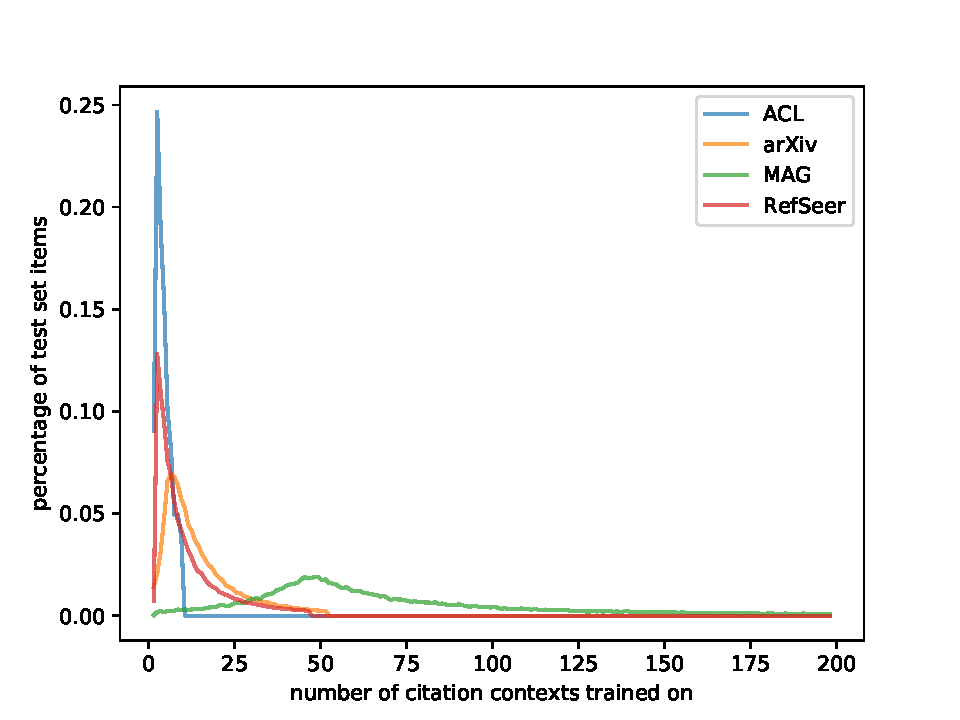
\includegraphics[width=.8\textwidth]{figures/evaluation/comparison_contexts_per_cited_doc.pdf}
  \caption{Number of citation contexts per recommendation candidate.}
  \label{fig:evalcomp}
\end{figure}

% In the following we will describe how the contexts were chosen from each of the data sets. In order to allow us to annotate\footnote{The calculation of NP and especially claim representations takes too much time to realisticly be done on the fly while learning and testing. These representations are therefore generated in a prior offline step.} and evaluate on several data sets with the available temporal and computational resources, we apply the following filter criteria to generate the data described in Table~\ref{tab:datasetprops}: arXiv contexts are those where the citing document is from the field of computer science and the cited document has at least 5 citing documents; MAG contexts are first filtered to be from the field of computer science, in English

The models used for recommendation are the four presented in Chapter~\ref{chap:approach}, ${R_{\text{FoS}}}$, ${R_{\text{NP}}}$, ${R_{\text{NPmrk}}^{2+}}$ and $R_{\text{claim}}$---which we will refer to as FoS, NP, NPmarker, and Claim from here on for simplicity---as well as a Bag-of-Words baseline (BoW) and two combined models (BoW+fosboost and Claim+BoW). The BoW baseline involves removal of punctuation as well as stopwords and uses TFIDF for ranking. We choose TFIDF over BM25 because the former shows better performance in our evaluations%
% \footnote{Maybe write a long footnote here about how BM25 gives comparable results to TFIDF when representations of cited documents are not jointly learned but contexts are treated separately, but this method in general gives worse results than using joinly learned representations}
. BoW+fosboost is constructed by taking the BoW ranking and then moving all candidates, where the overlap in fields of study (${\big|R_{\text{FoS}}(c_i)\cap\big(\bigcup\limits_{c \in \varrho(d)} R_{\text{FoS}}(c)\big)\big|}$, cf. Section~\ref{sec:approachfos}) is maximal, one position upwards in the ranking. Ranking in Claim+BoW is done by linearly combining similarity values $S(A,B)=\sum\limits_{m\in\mathcal{M}}\alpha_mS_m(A,B)$ of the models $\mathcal{M}=\{\text{Claim},\text{BoW}\}$ with heuristically determined coefficients $\alpha_{\text{Claim}}=1$ and $\alpha_{\text{BoW}}=2$.

Table~\ref{tab:arxivevalnumbers} shows NDCG, MAP, MRR and recall values at cut-off 5 for all models evaluated on the arXiv data. While FoS alone performs very poorly, the combined model BoW+fosboost consistently performs better then BoW alone. Nevertheless, because the performance gain is minute, we see no reason for a more detailed investigation of the models FoS and BoW+fosboost. Overall Claim+BoW shows the best performance, with NPmarker achieving the highest value for the MRR metric. To investigate the performance of these models further, we look at above metrics at different cut-off values and using multiple data sets. Note that arXiv is the only of our data sets where the NPmarker model is applicable (because the exact position of the citation marker is needed) and also the only of the data sets where more than one cited document in can be counted as relevant (cf. ``adjacent citations'' in Section~\ref{sec:datasetformat}).

% pre-filtering experiments (knn\cite{Bhagavatula2018}, lsi, lda, fos, ...)
% different evaluation settings (all, CSonly, comparison to MAG, ACL (data from \cite{Faerber2018b})...)
% FoS alone, restrictively combined w/ BOW, only directly preceeding, ...
% PP model alone, combined, ...

% -> not \emph{generally} applicable/beneficial but for certain citation types ...

% also mention \cite{Kobayashi2018} here b/c they specifically target cases where more than one citation is applicable (could be interpreted as either \emph{multiple (simultaneously)} for one context or \emph{several options that are all valid by themselves but in the end a single one is to be chosen} for one contexts)

\begin{table}[]
\centering
    \caption{Evaluation scores at cut-off 5 for all models using the arXiv data.}
    \label{tab:arxivevalnumbers}
\begin{center}
    \begin{tabular}{lllll}
    \toprule
    Model & NDCG@5 & MAP@5 & MRR@5 & Recall@5 \\
    \midrule
    Claim+BoW & \textbf{0.21829} & \textbf{0.34416} & 0.17530 & \textbf{0.27420} \\
    BoW+fosboost   & 0.20682 & 0.32980 & 0.16264 & 0.25824 \\
    BoW       & 0.20673 & 0.32961 & 0.16256 & 0.25817 \\
    NPmarker  & 0.17677 & 0.30769 & \textbf{0.17764} & 0.24931 \\
    Claim     & 0.08337 & 0.14441 & 0.07477 & 0.11750 \\
    NP        & 0.07914 & 0.13950 & 0.06775 & 0.10558 \\
    FoS       & 0.00921 & 0.01999 & 0.00420 & 0.00933 \\
    \bottomrule
    \end{tabular}
\end{center}
\end{table}

\begin{figure}
  \centering
    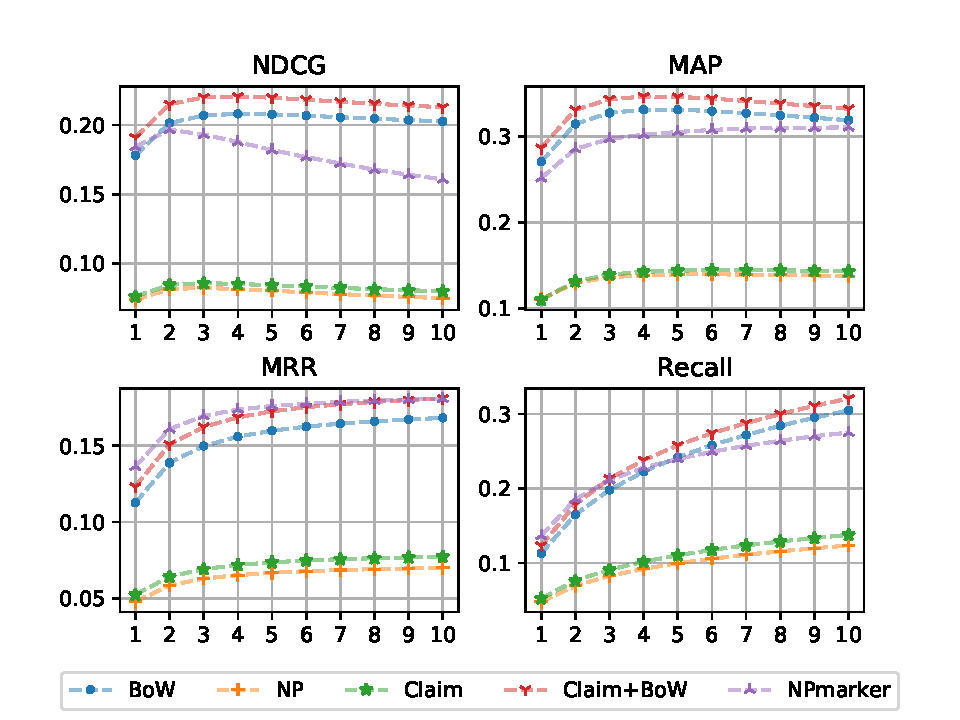
\includegraphics[width=.9\textwidth]{figures/evaluation/arXiv_CS_select.pdf}
  \caption{Evaluation using arXiv.}
  \label{fig:evalarxiv}
%\end{figure}

%\begin{figure}
  \centering
    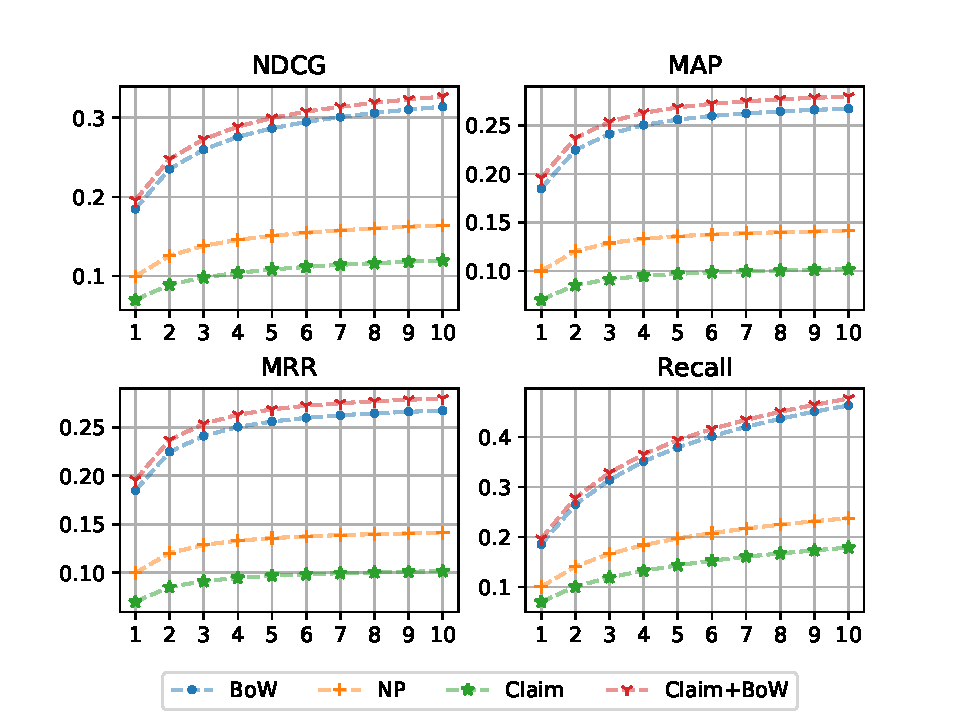
\includegraphics[width=.9\textwidth]{figures/evaluation/MAG_CS_en_wAbs.pdf}
  \caption{Evaluation using the MAG.}
  \label{fig:evalmag}
\end{figure}

\begin{figure}
  \centering
    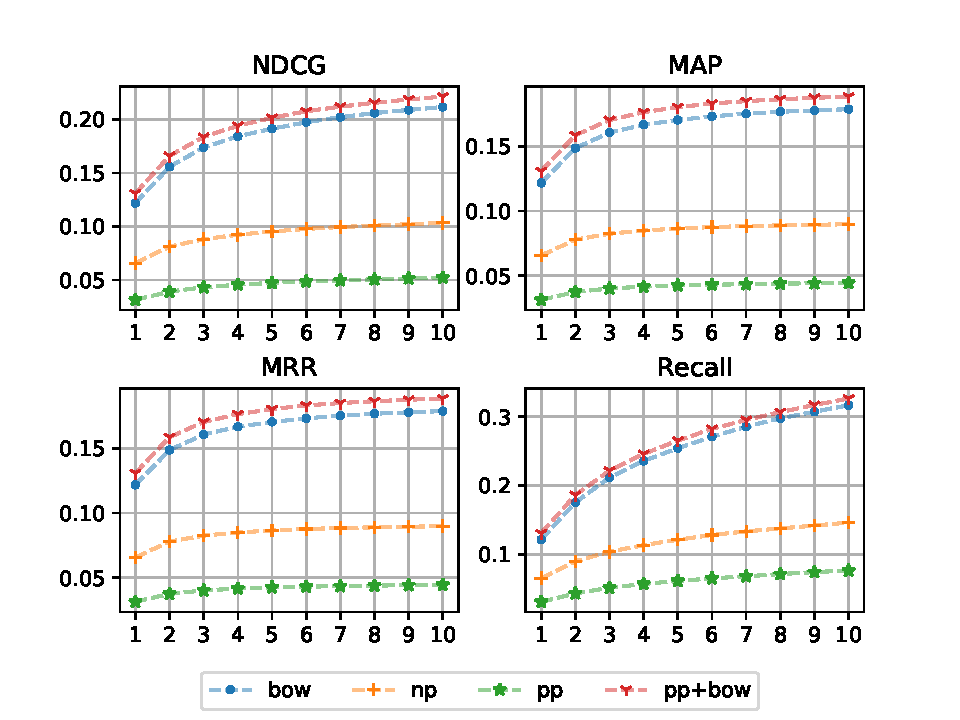
\includegraphics[width=.9\textwidth]{figures/evaluation/RefSeer.pdf}
  \caption{Evaluation using RefSeer.}
  \label{fig:evalrefseer}
%\end{figure}

%\begin{figure}
  \centering
    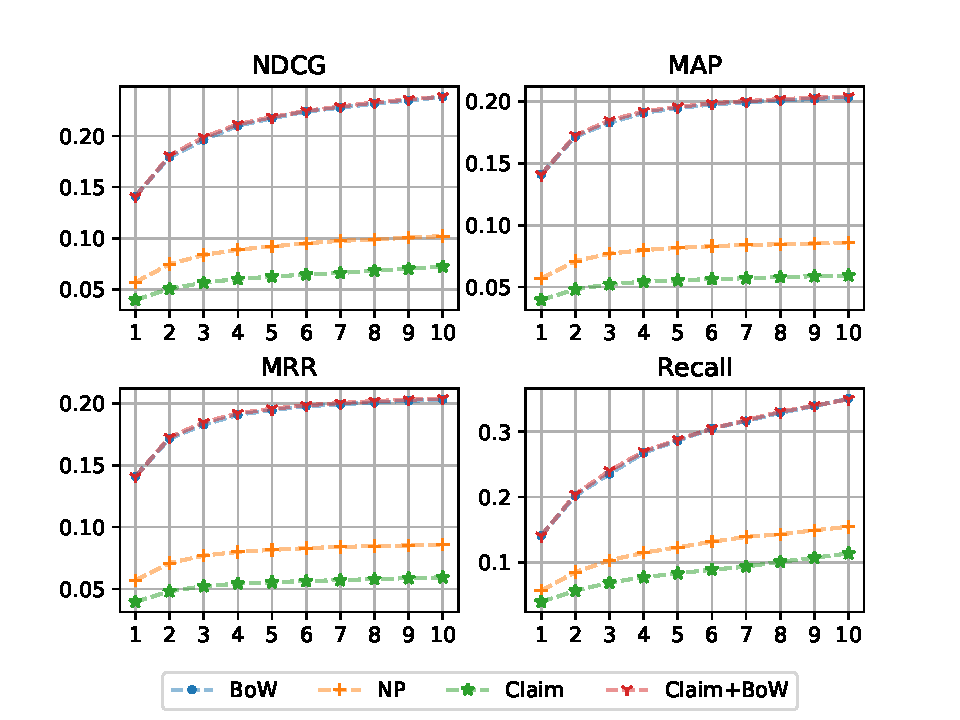
\includegraphics[width=.9\textwidth]{figures/evaluation/ACL.pdf}
  \caption{Evaluation using ACL-ARC.}
  \label{fig:evalacl}
\end{figure}

Figures~\ref{fig:evalarxiv}--\ref{fig:evalacl} show the results of these evaluations. For each of the data sets Claim+BoW outperforms the BoW baseline in each measure and for all cut-off values. Claim and NP do not compare in performance with the two aforementioned. This suggests that the claim structures we model with $R_{\text{claim}}$ are not enough for well performing recommendations on their own, but do capture information that non-semantic models (BoW) miss. NPmarker, only present in Figures~\ref{fig:evalarxiv}, gives particularly good results for lower cut-offs and performs especially well in the MRR metric. It performs the worst at high cut-offs measured by NDCG. Note that NPmarker is only evaluated for test set items where the model was applicable (i.e. where a noun phrase of minium length 2 is directly preceding the citation marker; cf. Section~\ref{sec:npmodel}). For our evaluation this was the case for 100,308 out of the 490,018 test set items (20.5\%). The evaluation results for NPmarker indicate that it is comparatively well suited to recommend citations where there is one particularly fitting publication (e.g. a reference paper for a tool, method or data set) and less suited for exemplifications (cf. Table~\ref{tab:citfunctions} in Chapter~\ref{chap:approach}). Comparing values between the different data sets, we can confirm our expectations based on the values in Table~\ref{tab:datasetprops}. For the MAG data, where we ensured very well described recommendation candidates by setting a threshold, the models perform best.
% Differences between the other three models are less straightforward, which is no surprise because there are many factors involved (number of recommendation candidates, number of contexts describing these, cleanliness of data, etc.).
This shows us that differences in data set composition can make a large difference in evaluation results. As a consequence, comparison between approaches is only realistically possible when using the same data.

% maybe mention \cite{Beel2017} ("None of these variations performed better than the simple out-of-the-box Apache Lucene baseline"), but then mention that Beel2017 is about *online* systems

% \cite{Huang2015} use CiteSeer\textsuperscript{x} (which RefSeer is based on) w/ 329,365 recommendation candidates. mby kind of comparable with a few buckets of salt?

\section{User study}\label{sec:oneval}
Main difference = direct human judgement

concerning author present criteria: can be unclear if author's name is part of NE (e.g. ``Pearson Correlation'')

\subsection{Non-free text}
(i.e. insight into offline eval)
(controlled for free text input bias)

\subsection{Free text}
free free
